%%
%% licence       kaneton licence
%%
%% project       kaneton
%%
%% file          /home/buckman/kaneton/view/books/assignments/k1.tex
%%
%% created       matthieu bucchianeri   [tue feb  7 11:49:38 2006]
%% updated       matthieu bucchianeri   [sun sep  3 17:50:50 2006]
%%

%
% k1
%

\chapter{k1}

The \textbf{k1} project consists in the development of the bootloader.

The bootloader, as the bootstrap, generally installs a better execution
environment for the future core execution.

Nevertheless, the main goal of the kaneton bootloader is to provide
information to the core on the current microprocessor's architecture
including the location of the pre-reserved physical memory areas etc..

This project is interesting since the student has to develop in a very
strict environment and build precise data structures which will be passed
to the core when launched.

\newpage

%
% informations
%

\section{Informations}

\begin{tabular}{p{7cm}l}
Duration: & One week \\
File name: & \textit{[group]}-k1.tar.gz \\
In charge: & Julien Quintard \\
Newgroup: & kaneton-students@googlegroups.com \\
Languages: & Assembly and C \\
Students per group: & Three \\
Target directories: & \textit{kaneton/bootloader/arch/[architecture]/} \\
\end{tabular}

%
% assignments
%

\section{Assignments}

In this project, the students have to develop the entire bootloader.
This means that no interface will be provided.

The only requirement is your bootloader to be compliant with the
initialization structure passed to the kaneton microkernel.

If this structure is not correctly built, then the kernel would not
be able to run.

Below are listed the bootloader's steps:

\begin{enumerate}
  \item
    The bootloader generally installs a more evolved memory addressing model,
    depending on the microprocessor's architecture.
  \item
    The bootloader relocates the stuff, if necessary, depending on the
    microprocessor's architecture. Then, the bootloader builds the
    initialization structure.

    The stuff includes:

    \begin{itemize}
      \item
	The kernel code.
      \item
	The modules.
      \item
	The pre-reserved core segments.
      \item
	The pre-reserved core regions.
      \item
	The kernel stack.
      \item
	The alloc survival area.
    \end{itemize}
  \item
    Then, the booloader prepares the kernel stack and calls the core
    providing it the complete initialization structure.
\end{enumerate}

The relocation is not really necessary but we wanted the students
to understand low-level programming and more especially programming
in a very strict environment with no fine-grain allocator provided.

The main goal of this project is to lead the students to understand the
project source organization. Indeed, a complete development environment
is provided; therefore, the students should learn to use system defines,
internal facilities, kaneton tools etc.. to develop more quickly.

%
% tips
%

\section{Tips}

Try to think about a very simple memory allocator delivering single
pages or contiguous areas. This allocator should help students to
allocate dynamic memory while evolving in a very strict environment.

The bootloader receives from the bootstrap a list of modules. We are
assuming that the core to launch is the first module of this list.

%
% additional work
%

\section{Additional Work}

To be able to debug, students should write a tiny console driver.

Try to make this driver code generic so you can reuse it in the next steps.

%
% ia32
%

\section{Intel Architecture 32-bit}

The bootloader is highly specific to the microprocessor's architecture
since its main roles are to:

\begin{itemize}
  \item
    Install new memory addressing models.
  \item
    Build the pre-reserved core segments area.
  \item
    Build the pre-reserved core regions area.
\end{itemize}

The other tasks are independent of the architecture.

We will so detail the three previous points.

%
% memory addressing models
%

\subsection{Memory Addressing Models}

Since the kaneton microkernel can be implemented for multiple
sub-architectures, different Intel memory addressing models can be used.

We will assume in this document that the students implementing the
Intel architecture are using the \textit{ia32-virtual} sub-architecture,
meaning that they are implementing the kaneton microkernel with true
virtual memory.

Students willing implement kaneton with other specific Intel architecture
facilities should be able to adapt the assignments to their case.

So, in the case of the \textit{ia32-virtual} architecture, the bootloader
has to install two memory addressing models:

\begin{enumerate}
  \item
    First, the protected mode even if the bootstrap maybe installed it
    before.

    Indeed, the bootloader needs to rebuild the protected mode to be sure
    it is installed and to be able to maintain it.
  \item
    Then, the paging mode to enable true virtual memory.
\end{enumerate}

We advise the student to install the protected mode, then to relocate the
stuff above the 16Mb and build the initialization structure and finally to install the
virtual memory before calling the kernel.

In this way, you will handle the hardest architecture problem, the virtual
memory, at the end, before performing the very last step, calling the kernel.

%
% core segments
%

\subsection{Core Segments}

The core segments area passed to the kernel by the bootloader via
the initialization structure is used to specify the microkernel the
physical memory areas which have to be marked as pre-reserved by the core.

These memory areas are memory areas to keep from being erased like the
kernel code, the kernel stack, the initialization structure, the modules,
the core segments area, the core regions area, the survival area but also
architecture-specific areas like the ISA memory area etc..

%
% core regions
%

\subsection{Core Regions}

The core regions area must contain everything necessary to describe
the future core virtual memory state.

In other words, the core regions represent the future virtual memory
state of the core. By \textit{future} we mean once the core's region
manager is fully initialized. Indeed, the core's region manager will
use the initialization structure and more precisly the core regions to
properly rebuild the virtual memory.

So, on the Intel sub-architectures, these core regions include the mapped
video memory, the kernel code, the kernel stack, the initialization
structure, the survival area and any additional Intel specific elements
like the Global Descriptor Table etc..

Notice that it might be smart not to include the first memory page in
the core regions so null pointers dereferencing will cause page faults.

%
% layout
%

\subsection{Layout}

Below is a sample physical memory layout for the Intel sub-architectures:

\begin{center}
  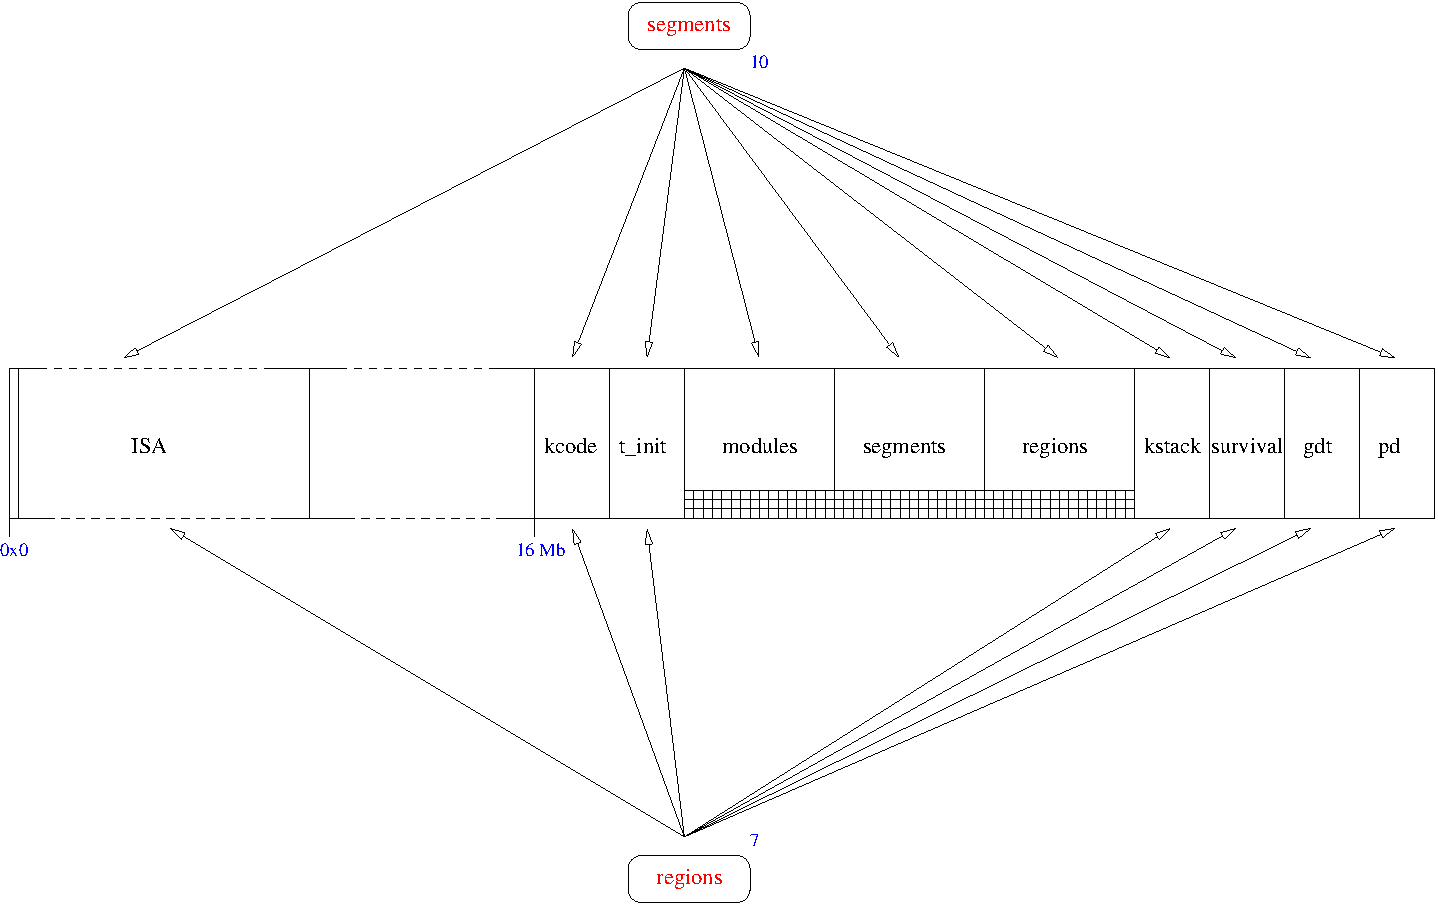
\includegraphics[scale=0.7]{figures/k1-memory-layout.pdf}
\end{center}
